\documentclass[12pt]{article}
\usepackage[T1, T2A]{fontenc}
\usepackage[utf8]{inputenc}
\usepackage{datetime}

\usepackage{amssymb}
\usepackage{amsmath}
\usepackage{amsfonts}

\usepackage{tikz}
\usetikzlibrary{shapes.geometric, arrows.meta, bending}

\tikzstyle{class} = [circle, text centered, draw, double, double distance=1.5pt, minimum width=1.5cm, minimum height=1.5cm]
\tikzstyle{instance} = [circle, text centered, draw, minimum width=1.5cm, minimum height=1.5cm]
\tikzstyle{arrow} = [thick,->,>=stealth]

\author{Grigorii Matiukhin}
\title{AI Methods Homeworks}

\begin{document}

\maketitle
\tableofcontents
\newpage

\section{Homework 1}

\subsection{Predicates}
\begin{itemize}
  \item \texttt{on\_top\_of(c1, c2)} --- Container \texttt{c1} is on top of \texttt{c2} 
  \item \texttt{on\_floor(c)} --- container \texttt{c} is on the floor 
  \item \texttt{topmost(c)} --- container \texttt{c} is at the top of the stack, even if it is the only one container in it 
  \item \texttt{bottommost(c)} --- container \texttt{c} is at the bottom of the stack, even if it is the only one container in it 
  \item \texttt{in\_stack(c, st)} --- container \texttt{c} is in stack \texttt{st} 
  \item \texttt{in\_gripper(c)} --- container \texttt{c} is in the gripper 
  \item \texttt{on\_ship(c)} --- container \texttt{c} is on ship 
  \item \texttt{gripper\_over\_stack(st)} --- Gripper is above the stack 
  \item \texttt{gripper\_empty} --- Whether gripper holds any containers 
  \item \texttt{gripper\_not\_empty} --- Whether gripper doesn't hold any containers 
  \item \texttt{gripper\_over\_ship(s)} --- Whether gripper is over a ship
\end{itemize}

\subsection{Rules}
\begin{itemize}
  \item \texttt{move\_gripper\_over\_stack(st, s)}
    \begin{itemize}
      \item C: \texttt{gripper\_empty}, \texttt{gripper\_over\_ship(s)}
      \item A: \texttt{gripper\_over\_stack(st)}
      \item D: \texttt{gripper\_over\_ship(s)}
    \end{itemize}
  \item \texttt{grab(c1, c2, st)}
    \begin{itemize}
      \item C: \texttt{gripper\_over\_stack(st)}, \texttt{topmost(c1)}, \texttt{in\_stack(c1, st)}, \texttt{in\_stack(c2, st)}, \texttt{gripper\_empty}, \texttt{on\_top\_of(c1, c2)}
      \item A: \texttt{in\_gripper(c)}, \texttt{gripper\_not\_empty}, \texttt{topmost(c2)}
      \item D: \texttt{in\_stack(c, st)}, \texttt{on\_top\_of(c1, c2)}, \texttt{topmost(c1)}
    \end{itemize}
  \item \texttt{grab\_bottommost(c, st)}
    \begin{itemize}
      \item C: \texttt{gripper\_over\_stack(st)}, \texttt{topmost(c)}, \texttt{in\_stack(c, st)}, \texttt{gripper\_empty}, \texttt{bottommost(c1)}
      \item A: \texttt{in\_gripper(c)}, \texttt{gripper\_not\_empty}, \texttt{topmost(c2)}
      \item D: \texttt{in\_stack(c, st)}, \texttt{topmost(c)}, \texttt{bottommost(c)}
    \end{itemize}
  \item \texttt{move\_gripper\_to\_ship(s, st)}
    \begin{itemize}
      \item C: \texttt{gripper\_not\_empty}, \texttt{gripper\_over\_stack(st)}
      \item A: \texttt{gripper\_over\_ship(s)}
      \item D: \texttt{gripper\_over\_stack(st)}
    \end{itemize}
  \item \texttt{drop\_container\_on\_ship(c, s)}
    \begin{itemize}
      \item C: \texttt{gripper\_not\_empty}, \texttt{in\_gripper(c)}, \texttt{gripper\_over\_ship(s)}
      \item A: \texttt{on\_ship(c)}
      \item D: \texttt{in\_gripper(c)}
    \end{itemize}
\end{itemize}

\subsection{Simulation}
\subsubsection{Given}
\begin{itemize}
  \item \texttt{in\_stack(c1, st1)}
  \item \texttt{in\_stack(c2, st1)}
  \item \texttt{in\_stack(c3, st1)}
  \item \texttt{in\_stack(c4, st2)}
  \item \texttt{in\_stack(c5, st2)}
  \item \texttt{topmost(c1)}
  \item \texttt{on\_top\_of(c1, c2)}
  \item \texttt{on\_top\_of(c2, c3)}
  \item \texttt{bottommost(c3)}
  \item \texttt{topmost(c4)}
  \item \texttt{on\_top\_of(c4, c5)}
  \item \texttt{bottommost(c5)}
  \item \texttt{gripper\_empty}
  \item \texttt{gripper\_over\_ship(s)}
\end{itemize}

\subsubsection{Goals}
\begin{itemize}
  \item \texttt{on\_ship(c1)}
  \item \texttt{on\_ship(c2)}
  \item \texttt{on\_ship(c3)}
  \item \texttt{on\_ship(c4)}
  \item \texttt{on\_ship(c5)}
  \item \texttt{gripper\_empty}
\end{itemize}

\subsection{Execution}
\begin{enumerate}
  \item Step 1:
    \begin{itemize}
      \item Conflict set: \texttt{move\_gripper\_over\_stack(st1, s)}, \texttt{move\_gripper\_over\_stack(st2, s)}
      \item Action: \texttt{move\_gripper\_over\_stack(st1, s)}
      \item Result:
        \begin{itemize}
          \item \texttt{in\_stack(c1, st1)}
          \item \texttt{in\_stack(c2, st1)}
          \item \texttt{in\_stack(c3, st1)}
          \item \texttt{in\_stack(c4, st2)}
          \item \texttt{in\_stack(c5, st2)}
          \item \texttt{topmost(c1)}
          \item \texttt{on\_top\_of(c1, c2)}
          \item \texttt{on\_top\_of(c2, c3)}
          \item \texttt{bottommost(c3)}
          \item \texttt{topmost(c4)}
          \item \texttt{on\_top\_of(c4, c5)}
          \item \texttt{bottommost(c5)}
          \item \texttt{gripper\_empty}
          \item \texttt{gripper\_over\_stack(st1)}
        \end{itemize}
    \end{itemize}
  \item Step 2:
    \begin{itemize}
      \item Conflict set: \texttt{grab(c1, c2, st1)}
      \item Action: \texttt{grab(c1, c2, st1)}
      \item Result:
        \begin{itemize}
          \item \texttt{in\_stack(c2, st1)}
          \item \texttt{in\_stack(c3, st1)}
          \item \texttt{in\_stack(c4, st2)}
          \item \texttt{in\_stack(c5, st2)}
          \item \texttt{topmost(c2)}
          \item \texttt{on\_top\_of(c1, c2)}
          \item \texttt{on\_top\_of(c2, c3)}
          \item \texttt{bottommost(c3)}
          \item \texttt{topmost(c4)}
          \item \texttt{on\_top\_of(c4, c5)}
          \item \texttt{bottommost(c5)}
          \item \texttt{gripper\_over\_stack(st1)}
          \item \texttt{in\_gripper(c1)}
          \item \texttt{gripper\_not\_empty}
        \end{itemize}
    \end{itemize}
  \item Step 3:
    \begin{itemize}
      \item Conflict set: \texttt{move\_gripper\_to\_ship(s, st1)}
      \item Action: \texttt{move\_gripper\_to\_ship(s, st1)}
      \item Result:
        \begin{itemize}
          \item \texttt{in\_stack(c2, st1)}
          \item \texttt{in\_stack(c3, st1)}
          \item \texttt{in\_stack(c4, st2)}
          \item \texttt{in\_stack(c5, st2)}
          \item \texttt{topmost(c2)}
          \item \texttt{bottommost(c3)}
          \item \texttt{on\_top\_of(c1, c2)}
          \item \texttt{on\_top\_of(c2, c3)}
          \item \texttt{topmost(c4)}
          \item \texttt{on\_top\_of(c4, c5)}
          \item \texttt{bottommost(c5)}
          \item \texttt{in\_gripper(c1)}
          \item \texttt{gripper\_not\_empty}
          \item \texttt{gripper\_over\_ship(s)}
        \end{itemize}
    \end{itemize}
  \item Step 4:
    \begin{itemize}
      \item Conflict set: \texttt{drop\_container\_on\_ship(c, s)}
      \item Action: \texttt{drop\_container\_on\_ship(c, s)}
      \item Result:
        \begin{itemize}
          \item \texttt{in\_stack(c2, st1)}
          \item \texttt{in\_stack(c3, st1)}
          \item \texttt{in\_stack(c4, st2)}
          \item \texttt{in\_stack(c5, st2)}
          \item \texttt{topmost(c2)}
          \item \texttt{on\_top\_of(c1, c2)}
          \item \texttt{on\_top\_of(c2, c3)}
          \item \texttt{bottommost(c3)}
          \item \texttt{topmost(c4)}
          \item \texttt{on\_top\_of(c4, c5)}
          \item \texttt{bottommost(c5)}
          \item \texttt{gripper\_empty}
          \item \texttt{gripper\_over\_ship(s)}
          \item \texttt{on\_ship(c1)}
        \end{itemize}
    \end{itemize}
\end{enumerate}
 

\newpage
\section{Homework 2}

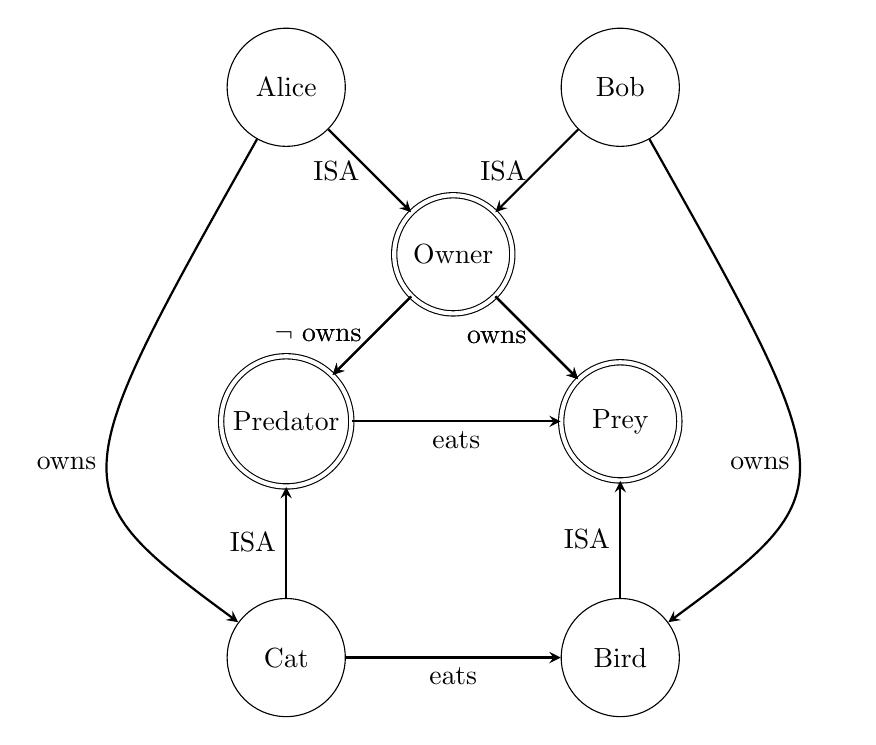
\begin{tikzpicture}[node distance=3cm]

  \node (owner) [class] {Owner};
  \node (predator) [class, below left of=owner] {Predator};
  \node (prey) [class, below right of=owner] {Prey};

  \node (alice) [instance, above left of=owner] {Alice};
  \node (bob) [instance, above right of=owner] {Bob};

  \node (cat) [instance, below of=predator] {Cat};
  \node (bird) [instance, below of=prey] {Bird};

  \draw [arrow] (owner) -- node[anchor=east] {owns} (predator);
  \draw [arrow] (owner) -- node[anchor=east] {owns} (prey);
  \draw [arrow] (predator) -- node[anchor=north] {eats} (prey);

  \draw [arrow] (alice) -- node[anchor=east] {ISA} (owner);
  \draw [arrow] (bob) -- node[anchor=east] {ISA} (owner);

  \draw [arrow] (owner) -- node[anchor=east] {$\neg$ owns} (predator);
  \draw [arrow] (owner) -- node[anchor=east] {owns} (prey);

  \draw [arrow] (alice) .. controls(-5, -3) .. node[anchor=east] {owns} (cat);
  \draw [arrow] (bob) .. controls(5, -3) .. node[anchor=east] {owns} (bird);

  \draw [arrow] (cat) -- node[anchor=east] {ISA} (predator);
  \draw [arrow] (bird) -- node[anchor=east] {ISA} (prey);
  \draw [arrow] (cat) -- node[anchor=north] {eats} (bird);

\end{tikzpicture}

\newpage
\section{Homework 3}
"Red sky at night, sailor's delight. Red sky in the morning, sailor's warning." \\
"Dew on the grass, no rain will come to pass." \\
"Seagull, seagull sit on the sand. It's never good weather when you're on land." \\
"A cow with its tail to the West makes the weather best, a cow with its tail to the East makes the weather least." \\
"When clouds look like black smoke a wise man will put on his cloak." \\
"No weather is ill if the wind be still." \\
"When halo rings the Moon or Sun, rain's approaching on the run."

\newpage
\section{Homework 4}

\subsection{Доказать с помощью метода резолюций, что формула $G$ есть логическое следствие формул $F_1,...,F_n$}
\subsubsection{а}
\begin{gather*}
  F_1 = X \vee Y, F_2 = X \rightarrow Z, G = \left( Y \rightarrow Z \right) \rightarrow Z \\
  \{X \vee Y, X \rightarrow Z, \overline{\left( Y \rightarrow Z \right) \rightarrow Z } \} \\
  \{X \vee Y, \overline{X} \vee Z, \overline{  \overline{ Y \rightarrow Z } \vee Z } \} \\
  \{X \vee Y, \overline{X} \vee Z, \overline{ \left( Y \wedge \overline{Z} \right) \vee Z } \} \\
  \{X \vee Y, \overline{X} \vee Z, \overline{ \left( Y \vee Z \right) \wedge \left( \overline{Z} \vee Z \right) } \} \\
  \{X \vee Y, \overline{X} \vee Z, \overline{ Y \vee Z } \} \\
  \{X \vee Y, \overline{X} \vee Z,  \overline{Y} \wedge \overline{Z} \} \\
  \{X \vee Y, \overline{X} \vee Z,  \overline{Y} \wedge \overline{Z} \} \\
  \{X \vee Y, \overline{X} \vee Z,  \overline{Y}, \overline{Z} \} \\
  \\
  \frac{X \vee Y, \overline{Y}}{X} \\
  \{X \vee Y, \overline{X} \vee Z,  \overline{Y}, \overline{Z}, X \} \\
  \\
  \frac{\overline{X} \vee Z, X}{Z} \\
  \{X \vee Y, \overline{X} \vee Z,  \overline{Y}, \overline{Z}, X, Z \} \\
  \\
  \frac{\overline{Z}, Z}{\emptyset} \\
\end{gather*}

\subsubsection{б}
\begin{gather*}
  F_1 = X, F_2 = X \wedge Y \rightarrow Z, G = Y \rightarrow Z \\
  \{X, X \wedge Y \rightarrow Z,  \overline{ Y \rightarrow Z }\} \\
  \{X, \overline{ X \wedge Y } \vee Z, \overline {\overline{Y} \vee Z }\} \\
  \{X, \overline{X} \vee \overline{Y} \vee Z, Y \wedge \overline{Z}\} \\
  \{X, \overline{X} \vee \overline{Y} \vee Z, Y, \overline{Z}\} \\
  \\
  \frac{X, \overline{X} \vee \overline{Y} \vee Z}{\overline{Y} \vee Z} \\
  \{X, \overline{X} \vee \overline{Y} \vee Z, Y, \overline{Z}, \overline{Y} \vee Z\} \\
  \\
  \frac{Y, \overline{Y} \vee Z}{Z} \\
  \{X, \overline{X} \vee \overline{Y} \vee Z, Y, \overline{Z}, \overline{Y} \vee Z, Z\} \\
  \\
  \frac{\overline{Z}, Z}{\emptyset} \\
\end{gather*}

\subsubsection{в}
\begin{gather*}
  F_1 = X \rightarrow Y \vee Z, F_2 = Z \rightarrow W, F_3 = \overline{W}, G = X \rightarrow Y \\
  \{ X \rightarrow Y \vee Z, Z \rightarrow W, \overline{W}, \overline{ X \rightarrow Y} \} \\
  \{ \overline{X} \vee Y \vee Z, \overline{Z} \vee W, \overline{W}, \overline{ \overline{X} \vee Y} \} \\
  \{ \overline{X} \vee Y \vee Z, \overline{Z} \vee W, \overline{W}, X \wedge \overline{Y} \} \\
  \{ \overline{X} \vee Y \vee Z, \overline{Z} \vee W, \overline{W}, X, \overline{Y} \} \\
  \\
  \frac{\overline{Z} \vee W, \overline{W}}{\overline{Z}} \\
  \{ \overline{X} \vee Y \vee Z, \overline{Z} \vee W, \overline{W}, X, \overline{Y}, \overline{Z} \} \\
  \\
  \frac{\overline{X} \vee Y \vee Z, X}{Y \vee Z} \\
  \{ \overline{X} \vee Y \vee Z, \overline{Z} \vee W, \overline{W}, X, \overline{Y}, \overline{Z}, Y \vee Z \} \\
  \\
  \frac{\overline{Z}, Y \vee Z}{Y} \\
  \{ \overline{X} \vee Y \vee Z, \overline{Z} \vee W, \overline{W}, X, \overline{Y}, \overline{Z}, Y \vee Z, Y\} \\
  \\
  \frac{\overline{Y}, Y}{\emptyset} \\
\end{gather*}

\subsubsection{г}
\begin{gather*}
  F_1 = X \vee Y \vee \neg Z, F_2 = X \rightarrow X_1, F_3 = Y \rightarrow Y_1, F_4 = Z, G = X_1 \vee Y_1 \\
  \{X \vee Y \vee \overline{Z}, X \rightarrow X_1, Y \rightarrow Y_1, Z, \overline{X_1 \vee Y_1}\} \\
  \{X \vee Y \vee \overline{Z}, \overline{X} \vee X_1, \overline{Y} \vee Y_1, Z, \overline{X_1} \wedge \overline{Y_1}\} \\
  \{X \vee Y \vee \overline{Z}, \overline{X} \vee X_1, \overline{Y} \vee Y_1, Z, \overline{X_1}, \overline{Y_1}\} \\
  \\
  \frac{\overline{X} \vee X_1, \overline{X_1}}{\overline{X}} \\
  \{X \vee Y \vee \neg \overline{Z}, \overline{X} \vee X_1, \overline{Y} \vee Y_1, Z, \overline{X_1}, \overline{Y_1}, \overline{X}\} \\
  \\
  \frac{\overline{Y} \vee Y_1, \overline{Y_1}}{\overline{Y}} \\
  \{X \vee Y \vee \overline{Z}, \overline{X} \vee X_1, \overline{Y} \vee Y_1, Z, \overline{X_1}, \overline{Y_1}, \overline{X}, \overline{Y}\} \\
  \\
  \frac{X \vee Y \vee \overline{Z}, \overline{X}}{Y \vee \overline{Z}} \\
  \{X \vee Y \vee \overline{Z}, \overline{X} \vee X_1, \overline{Y} \vee Y_1, Z, \overline{X_1}, \overline{Y_1}, \overline{X}, \overline{Y}, Y \vee \overline{Z}\} \\
  \\
  \frac{Y \vee \overline{Z}, Z}{Y} \\
  \{X \vee Y \vee \overline{Z}, \overline{X} \vee X_1, \overline{Y} \vee Y_1, Z, \overline{X_1}, \overline{Y_1}, \overline{X}, \overline{Y}, Y \vee \overline{Z}, Y\} \\
  \\
  \frac{Y, \overline{Y}}{\emptyset} \\
\end{gather*}

\subsubsection{д}
\begin{gather*}
  F_1 = X Y \rightarrow \overline{X}Z, F_2 = \overline{X \overline{Y}} \vee Z, G = X \rightarrow Z \\
  \{XY \rightarrow \overline{X}Z, \overline{X \overline{Y}} \vee Z, \overline{X \rightarrow Z}\} \\
  \{\overline{XY} \vee \overline{X}Z, \overline{X} \vee Y \vee Z, \overline{\overline{X} \vee Z}\} \\
  \{\overline{XY \wedge \overline{\overline{X}Z}}, \overline{X} \vee Y \vee Z, X \wedge \overline{Z}\} \\
  \{\overline{XY \wedge X \vee \overline{Z}}, \overline{X} \vee Y \vee Z, X, \overline{Z}\} \\
  \{\overline{XYX \vee XY\overline{Z}}, \overline{X} \vee Y \vee Z, X, \overline{Z}\} \\
  \{\overline{XY \vee XY\overline{Z}}, \overline{X} \vee Y \vee Z, X, \overline{Z}\} \\
  \{\overline{XY \left(1\vee \overline{Z}\right)}, \overline{X} \vee Y \vee Z, X, \overline{Z}\} \\
  \{\overline{XY}, \overline{X} \vee Y \vee Z, X, \overline{Z}\} \\
  \{\overline{X} \vee \overline{Y}, \overline{X} \vee Y \vee Z, X, \overline{Z}\} \\
  \\
  \frac{\overline{X} \vee \overline{Y}, X}{\overline{Y}} \\
  \{\overline{X} \vee \overline{Y}, \overline{X} \vee Y \vee Z, X, \overline{Z}, \overline{Y}\} \\
  \\
  \frac{\overline{X} \vee Y \vee Z, \overline{Y}}{\overline{X} \vee Z} \\
  \{\overline{X} \vee \overline{Y}, \overline{X} \vee Y \vee Z, X, \overline{Z}, \overline{Y}, \overline{X} \vee Z\} \\
  \\
  \frac{\overline{Z}, \overline{X} \vee Z}{\overline{X}} \\
  \{\overline{X} \vee \overline{Y}, \overline{X} \vee Y \vee Z, X, \overline{Z}, \overline{Y}, \overline{X} \vee Z, \overline{X}\} \\
  \\
  \frac{\overline{X}, X}{\emptyset} \\
\end{gather*}

\subsubsection{е}
\begin{gather*}
  F_1 = X \rightarrow \left( \overline{Y}\left( \overline{Y} \rightarrow Z \right)\right), F_2 = \left(X \rightarrow \overline{Y}\right) \wedge \overline{\left(\overline{X} \wedge \overline{W}\right)}, G = W \vee Z \\
  \{X \rightarrow \left( \overline{Y}\left( \overline{Y} \rightarrow Z \right)\right), \left(X \rightarrow \overline{Y}\right) \wedge \overline{\left(\overline{X} \wedge \overline{W}\right)}, \overline{W \vee Z}\} \\
  \{X \rightarrow \left( \overline{Y}\left( Y \vee Z \right)\right), \left(\overline{X} \vee \overline{Y}\right) \wedge \left(X \vee W \right), \overline{W} \wedge \overline{Z}\} \\
  \{\overline{X} \vee \overline{Y}Y \vee \overline{Y}Z, \overline{X} \vee \overline{Y}, X \vee W, \overline{W}, \overline{Z}\} \\
  \{\overline{X} \vee \overline{Y}Z, \overline{X} \vee \overline{Y}, X \vee W, \overline{W}, \overline{Z}\} \\
  \{\left(\overline{X} \vee \overline{Y} \right) \wedge \left(\overline{X} \vee Z \right), \overline{X} \vee \overline{Y}, X \vee W, \overline{W}, \overline{Z}\} \\
  \{\overline{X} \vee \overline{Y}, \overline{X} \vee Z, \overline{X} \vee \overline{Y}, X \vee W, \overline{W}, \overline{Z}\} \\
  \\
  \frac{X \vee W, \overline{W}}{X} \\
  \{\overline{X} \vee \overline{Y}, \overline{X} \vee Z, \overline{X} \vee \overline{Y}, X \vee W, \overline{W}, \overline{Z}, X\} \\
  \\
  \frac{\overline{X} \vee Z, X}{Z} \\
  \{\overline{X} \vee \overline{Y}, \overline{X} \vee Z, \overline{X} \vee \overline{Y}, X \vee W, \overline{W}, \overline{Z}, X, Z\} \\
  \\
  \frac{\overline{Z}, Z}{\emptyset} \\
\end{gather*}

\subsection{Доказать с помощью метода резолюций, что формула $G$ есть логическое следствие формул $F_1,...,F_n$ }
\subsubsection{а}
\begin{gather*}
  F_1 = \left(\forall x\right)\left(P(x)\rightarrow Q(x)R(X)\right), \\
  F_2 = \left(\exists x\right)\left(P(x)T(x)\right), \\
  G = \left(\exists x\right)\left(R(x)T(x)\right) \\
  \\
  \{\left(\forall x\right)\left(P(x)\rightarrow Q(x)R(x)\right), \left(\exists x\right)\left(P(x)T(x)\right), \neg\left(\exists x\right)\left(R(x)T(x)\right)\} \\
  \{\left(\forall x\right)\left(\neg P(x)\vee Q(x)R(x)\right), P(f)T(f), \left(\forall\right)\neg\left(R(x)T(x)\right)\} \\
  \{\left(\forall x\right)\left(\left(\neg P(x)\vee Q(x)\right)\wedge\left(\neg P(x) \vee R(x)\right)\right), P(f), T(f), \left(\forall\right)\left(\neg R(x)\vee \neg T(x)\right)\} \\
  \{\neg P(x)\vee Q(x), \neg P(x) \vee R(x), P(f), T(f), \neg R(x)\vee \neg T(x)\} \\
  \\
  \frac{\neg P(x) \vee R(x), \neg R(x) \vee \neg T(x)}{\neg P(x) \vee \neg T(x)} \\
  \{\neg P(x)\vee Q(x), \neg P(x) \vee R(x), P(f), T(f), \neg R(x)\vee \neg T(x), \neg P(x) \vee \neg T(x)\} \\
  \\
  \frac{\neg P(x) \vee \neg T(x), T(f)}{\neg P(f)}\left[x/f\right] \\
  \{\neg P(x)\vee Q(x), \neg P(x) \vee R(x), P(f), T(f), \neg R(x)\vee \neg T(x), \neg P(x) \vee \neg T(x), \neg P(f)\} \\
  \\
  \frac{P(f), \neg P(f)}{\emptyset} \\
\end{gather*}

\subsubsection{б}
\begin{gather*}
  F_1 = \left(\forall x\right)\left[\left(\exists y\right)\left(M(y)S(x,y)\right) \rightarrow \left(\exists z\right)\left(I(z)E(x,z)\right)\right], \\
  G = \neg \left(\exists x\right)I(x)\rightarrow \left(\forall u\right)\left(\forall v\right)\left(S(u, v) \rightarrow \neg M(v)\right) \\
  \left\{
    \begin{array}{c}
  \left(\forall x\right)\left[\left(\exists y\right)\left(M(y)S(x,y)\right) \rightarrow \left(\exists z\right)\left(I(z)E(x,z)\right)\right], \\
  \neg \left(\neg \left(\exists x\right)I(x)\rightarrow \left(\forall u\right)\left(\forall v\right)\left(S(u, v) \rightarrow \neg M(v)\right)\right)
    \end{array}
  \right\} \\
  \left\{
    \begin{array}{c}
  \left(\forall x\right)\left[\neg\left(\exists y\right)\left(M(y)S(x,y)\right) \vee \left(\exists z\right)\left(I(z)E(x,z)\right)\right], \\
    \neg \left(\left(\exists x\right)I(x)\vee \left(\forall u\right)\left(\forall v\right)\left(\neg S(u, v) \vee \neg M(v)\right)\right)
    \end{array}
  \right\} \\
  \left\{
    \begin{array}{c}
      \left(\forall x\right)\left[\left(\forall y\right)\neg\left(M(y)S(x,y)\right) \vee \left(\exists z\right)\left(I(z)E(x,z)\right)\right], \\
    \neg\left(\exists x\right)I(x)\wedge \neg\left(\left(\forall u\right)\left(\forall v\right)\neg\left(S(u, v) \wedge M(v)\right)\right)
    \end{array}
  \right\} \\
  \left\{
    \begin{array}{c}
      \left(\forall x\right)\left(\forall y\right)\left(\exists z\right)\left[\neg\left(M(y)S(x,y)\right) \vee \left(I(z)E(x,z)\right)\right], \\
      \left(\forall x\right)\neg I(x)\wedge \left(\left(\exists u\right)\left(\exists v\right)\left(S(u, v) \wedge M(v)\right)\right)
    \end{array}
  \right\} \\
  \left\{
    \begin{array}{c}
      \left(\forall x\right)\left(\forall y\right)\left(\exists z\right)\left[\neg\left(M(y)S(x,y)\right) \vee \left(I(z)E(x,z)\right)\right], \\
      \left(\forall x\right)\neg I(x)\wedge \left(\left(\exists u\right)\left(\exists v\right)\left(S(u, v) \wedge M(v)\right)\right)
    \end{array}
  \right\} \\
  \left\{
    \begin{array}{c}
      \left(\forall x\right)\left(\forall y\right)\left(\exists z\right)\left[\neg M(y) \vee \neg S(x,y) \vee \left(I(z)E(x,z)\right)\right], \\
      \left(\forall x\right)\left(\exists u\right)\left(\exists v\right)\left(\neg I(x)\wedge S(u, v) \wedge M(v)\right)
    \end{array}
  \right\} \\
  \left\{
    \begin{array}{c}
      \left(\forall x\right)\left(\forall y\right)\left(\exists z\right)\left[\left(\neg M(y) \vee \neg S(x,y) \vee I(z)\right) \wedge \left(\neg M(y) \vee \neg S(x,y) \vee E(x,z)\right)\right], \\
      \left(\forall x\right)\left(\neg I(x)\wedge S(f(x), g(x)) \wedge M(g(x))\right)
    \end{array}
  \right\} \\
  \left\{
    \begin{array}{c}
      \left(\forall x\right)\left(\forall y\right)\left[\left(\neg M(y) \vee \neg S(x,y) \vee I(f(x, y))\right) \wedge \left(\neg M(y) \vee \neg S(x,y) \vee E(x,f(x, y))\right)\right], \\
      \left(\forall x\right)\left(\neg I(x)\wedge S(f(x), g(x)) \wedge M(g(x))\right)
    \end{array}
  \right\} \\
  \left\{
    \begin{array}{c}
      \neg M(y) \vee \neg S(x,y) \vee I(f(x,y)), \\
      \neg M(y) \vee \neg S(x,y) \vee E(x,f(x,y)), \\
      \neg I(x), S(f(x), g(x)), M(g(x))
    \end{array}
  \right\} \\
  \\
  \frac{\neg M(y) \vee \neg S(x, y) \vee I(f(x, y)), M(g(x))}{\neg S(x, y) \vee I(f(x, y))}\left[y/g(x)\right] \\
  \left\{
    \begin{array}{c}
      \neg M(y) \vee \neg S(x,y) \vee I(f(x,y)), \\
      \neg M(y) \vee \neg S(x,y) \vee E(x,f(x,y)), \\
      \neg I(x), S(f(x), g(x)), M(g(x)), \\
      \neg S(x, y) \vee I(f(x, y))
    \end{array}
  \right\} \\
  \\
  \frac{\neg S(x, y) \vee I(f(x, y)), S(x, y)}{I(f(x, y))} \\
  \left\{
    \begin{array}{c}
      \neg M(y) \vee \neg S(x,y) \vee I(f(x,y)), \\
      \neg M(y) \vee \neg S(x,y) \vee E(x,f(x,y)), \\
      \neg I(x), S(f(x), g(x)), M(g(x)), \\
      \neg S(x, y) \vee I(f(x, y)), I(f(x, y))
    \end{array}
  \right\} \\
  \\
  \frac{I(f(x, y)), \neg I(x)}{\emptyset}\left[x/f(x, y)\right]
\end{gather*}

\subsubsection{в}
\begin{gather*}
  F_1 = \left(\forall x\right)\left[P(x) \rightarrow \left(\exists y\right)\left(Q(y)S(x, y)\right)\right], \\
  F_2 = \left(\exists x\right)\left[R(x)\wedge\left(\forall y\right)\left(Q(y)\rightarrow S(x,y)\right)\right], \\
  F_3 = \left(\exists x\right)P(x), \\
  G = \left(\exists x\right)\left(\neg P(x) \vee R(x)\right) \\
  \left\{
    \begin{array}{c}
      \left(\forall x\right)\left[P(x) \rightarrow \left(\exists y\right)\left(Q(y)S(x, y)\right)\right], \\
      \left(\exists x\right)\left[R(x)\wedge\left(\forall y\right)\left(Q(y)\rightarrow S(x,y)\right)\right], \\
      \left(\exists x\right)P(x), \\
      \neg\left(\left(\exists x\right)\left(\neg P(x) \vee R(x)\right)\right) \\
    \end{array}
  \right\} \\
  \left\{
    \begin{array}{c}
      \left(\forall x\right)\left[\neg P(x) \vee \left(\exists y\right)\left(Q(y)S(x, y)\right)\right], \\
      \left(\exists x\right)\left[R(x)\wedge\left(\forall y\right)\left(\neg Q(y)\vee S(x,y)\right)\right], \\
      P(f), \\
      \left(\forall x\right)\neg\left(\neg P(x) \vee R(x)\right) \\
    \end{array}
  \right\} \\
  \left\{
    \begin{array}{c}
      \left(\forall x\right)\left(\exists y\right)\left[\neg P(x) \vee \left(Q(y)S(x, y)\right)\right], \\
      \left(\exists x\right)\left(\forall y\right)\left[R(x)\wedge\left(\neg Q(y)\vee S(x,y)\right)\right], \\
      P(f), \\
      \left(\forall x\right)\left(P(x) \wedge \neg R(x)\right) \\
    \end{array}
  \right\} \\
  \left\{
    \begin{array}{c}
      \left(\forall x\right)\left(\exists y\right)\left[\left(\neg P(x) \vee Q(y)\right)\wedge\left(\neg P(x) \vee S(x, y)\right)\right], \\
      \left(\forall y\right)\left[R(g)\wedge\left(\neg Q(y)\vee S(g,y)\right)\right], \\
      P(f), \\
      P(x), \neg R(x) \\
    \end{array}
  \right\} \\
  \left\{
    \begin{array}{c}
      \left(\forall x\right)\left[\left(\neg P(x) \vee Q(w(x))\right)\wedge\left(\neg P(x) \vee S(x, w(x))\right)\right], \\
      R(g), \neg Q(y)\vee S(g,y), \\
      P(f), \\
      P(x), \neg R(x) \\
    \end{array}
  \right\} \\
  \left\{
    \begin{array}{c}
      \neg P(x) \vee Q(w(x)), \neg P(x) \vee S(x, w(x)), \\
      R(g), \neg Q(y)\vee S(g,y), \\
      P(f), \\
      P(x), \neg R(x) \\
    \end{array}
  \right\} \\
  \\
  \frac{R(g), \neg R(x)}{\emptyset}\left[x/g\right]
\end{gather*}

\newpage
\section{Homework 5}
\subsection{Conditions}
\begin{itemize}
  \item \texttt{adjacent(r1, r2)}
  \item \texttt{box\_in(b, r)}
  \item \texttt{on\_floor(b)}
  \item \texttt{topmost(b)}
  \item \texttt{light\_off(r)}
  \item \texttt{light\_on(r)}
  \item \texttt{in(r)}
  \item \texttt{on\_top(b1, b2)}
  \item \texttt{holding{b}}
\end{itemize}

\subsection{Actions}
\begin{itemize}
  \item \texttt{step(r1, r2)}
    \begin{itemize}
      \item Preconditions: \texttt{in(r1)}, \texttt{adjacent(r1, r2)}
      \item Result: \texttt{in(r2)}
    \end{itemize}
  \item \texttt{pick\_in\_room(r, b1, b2)}
    \begin{itemize}
      \item Preconditions: \texttt{in(r)}, \texttt{box\_in(b1, r)}, \texttt{box\_in(b2, r)}, \texttt{on\_top(b1, b2)}, \texttt{topmost(b1)}
      \item Result: \texttt{not topmost(b1)}, \texttt{topmost(b2)}, \texttt{holding(b1)}
    \end{itemize}
  \item \texttt{pick\_floor(r, b)}
    \begin{itemize}
      \item Preconditions: \texttt{in(r)}, \texttt{box\_in(b1, r)}, \texttt{on\_floor(b1)}, \texttt{topmost(b1)}
      \item Result: \texttt{not topmost(b1)}, \texttt{holding(b1)}
    \end{itemize}
  \item \texttt{drop(r, b)}
    \begin{itemize}
      \item Preconditions: \texttt{in(r)}, \texttt{holding(b)}
      \item Result: \texttt{topmost(b)}, \texttt{on\_floor(b)}, \texttt{not holding(b)}
    \end{itemize}
  \item \texttt{turn\_on\_light(r, b)}
    \begin{itemize}
      \item Preconditions: \texttt{in(r)}, \texttt{on\_floor(b)}, \texttt{topmost(b)}, \texttt{light\_off(r)}
      \item Result: \texttt{light\_on(r)}
    \end{itemize}
\end{itemize}

\subsection{Given}
\begin{itemize}
  \item \texttt{box\_in(A, 3)}
  \item \texttt{box\_in(B, 3)}
  \item \texttt{box\_in(C, 3)}
  \item \texttt{box\_in(D, 3)}
  \item \texttt{on\_floor(A)}
  \item \texttt{on\_top(B, A)}
  \item \texttt{topmost(B)}
  \item \texttt{on\_floor(D)}
  \item \texttt{on\_top(C, D)}
  \item \texttt{topmost(C)}
  \item \texttt{light\_off(1)}
  \item \texttt{light\_off(2)}
  \item \texttt{light\_off(3)}
  \item \texttt{in(2)}
\end{itemize}

\subsubsection{Always}
\begin{itemize}
  \item \texttt{adjacent(1,4)}
  \item \texttt{adjacent(2,4)}
  \item \texttt{adjacent(3,4)}
  \item \texttt{adjacent(4,1)}
  \item \texttt{adjacent(4,2)}
  \item \texttt{adjacent(4,3)}
\end{itemize}

\subsection{Goals}
\begin{itemize}
  \item \texttt{in(2)}
  \item \texttt{light\_on(1)}
  \item \texttt{light\_on(2)}
  \item \texttt{light\_on(3)}
  \item \texttt{box\_in(A, 1)}
  \item \texttt{box\_in(C, 1)}
  \item \texttt{box\_in(B, 3)}
  \item \texttt{box\_in(D, 3)}
  \item \texttt{on\_floor(B)}
  \item \texttt{topmost(B)}
  \item \texttt{on\_floor(D)}
  \item \texttt{topmost(D)}
  \item \texttt{on\_top(A, C)}
  \item \texttt{on\_floor(C)}
  \item \texttt{topmost(A)}
\end{itemize}

\subsection{Execution}
\begin{enumerate}
  \item \texttt{light\_on(1)}
    \begin{itemize}
      \item Goals:
        \begin{enumerate}
          \item \texttt{in(2)} +
          \item \texttt{light\_on(1)} --
          \item \texttt{light\_on(2)} --
          \item \texttt{light\_on(3)} --
          \item \texttt{box\_in(A, 1)} --
          \item \texttt{box\_in(C, 1)} --
          \item \texttt{box\_in(B, 3)} +
          \item \texttt{box\_in(D, 3)} +
          \item \texttt{on\_floor(B)} --
          \item \texttt{topmost(B)} +
          \item \texttt{on\_floor(D)} +
          \item \texttt{topmost(D)} --
          \item \texttt{on\_top(A, C)} --
          \item \texttt{on\_floor(C)} --
          \item \texttt{topmost(A)} --
        \end{enumerate}
      \item Steps:
        \begin{enumerate}
          \item \texttt{step(2, 4)}
          \item \texttt{step(4, 3)}
          \item \texttt{pick\_in\_room(3, B, A)}
          \item \texttt{step(3, 4)}
          \item \texttt{step(4, 1)}
          \item \texttt{drop(1, B)}
          \item \texttt{turn\_on\_light(1, B)}
        \end{enumerate}
      \item State:
        \begin{itemize}
          \item \texttt{box\_in(A, 3)}
          \item \texttt{box\_in(B, 1)}
          \item \texttt{box\_in(C, 3)}
          \item \texttt{box\_in(D, 3)}
          \item \texttt{on\_floor(A)}
          \item \texttt{topmost(A)}
          \item \texttt{topmost(B)}
          \item \texttt{on\_floor(B)}
          \item \texttt{on\_floor(D)}
          \item \texttt{on\_top(C, D)}
          \item \texttt{topmost(C)}
          \item \texttt{light\_on(1)}
          \item \texttt{light\_off(2)}
          \item \texttt{light\_off(3)}
          \item \texttt{in(1)}
        \end{itemize}
    \end{itemize}
  \item \texttt{in(2)}
    \begin{itemize}
      \item Goals:
        \begin{enumerate}
          \item \texttt{in(2)} --
          \item \texttt{light\_on(1)} +
          \item \texttt{light\_on(2)} --
          \item \texttt{light\_on(3)} --
          \item \texttt{box\_in(A, 1)} --
          \item \texttt{box\_in(C, 1)} --
          \item \texttt{box\_in(B, 3)} --
          \item \texttt{box\_in(D, 3)} +
          \item \texttt{on\_floor(B)} +
          \item \texttt{topmost(B)} +
          \item \texttt{on\_floor(D)} +
          \item \texttt{topmost(D)} --
          \item \texttt{on\_top(A, C)} --
          \item \texttt{on\_floor(C)} --
          \item \texttt{topmost(A)} +
        \end{enumerate}
      \item Steps:
        \begin{enumerate}
          \item \texttt{step(1, 4)}
          \item \texttt{step(4, 2)}
        \end{enumerate}
      \item State:
        \begin{itemize}
          \item \texttt{box\_in(A, 3)}
          \item \texttt{box\_in(B, 1)}
          \item \texttt{box\_in(C, 3)}
          \item \texttt{box\_in(D, 3)}
          \item \texttt{on\_floor(A)}
          \item \texttt{topmost(A)}
          \item \texttt{topmost(B)}
          \item \texttt{on\_floor(B)}
          \item \texttt{on\_floor(D)}
          \item \texttt{on\_top(C, D)}
          \item \texttt{topmost(C)}
          \item \texttt{light\_on(1)}
          \item \texttt{light\_off(2)}
          \item \texttt{light\_off(3)}
          \item \texttt{in(2)}
        \end{itemize}
    \end{itemize}
  \item \texttt{light\_on(2)}
    \begin{itemize}
      \item Goals:
        \begin{enumerate}
          \item \texttt{in(2)} +
          \item \texttt{light\_on(1)} +
          \item \texttt{light\_on(2)} --
          \item \texttt{light\_on(3)} --
          \item \texttt{box\_in(A, 1)} --
          \item \texttt{box\_in(C, 1)} --
          \item \texttt{box\_in(B, 3)} --
          \item \texttt{box\_in(D, 3)} +
          \item \texttt{on\_floor(B)} +
          \item \texttt{topmost(B)} +
          \item \texttt{on\_floor(D)} +
          \item \texttt{topmost(D)} --
          \item \texttt{on\_top(A, C)} --
          \item \texttt{on\_floor(C)} --
          \item \texttt{topmost(A)} +
        \end{enumerate}
      \item Steps:
        \begin{enumerate}
          \item \texttt{step(2, 4)}
          \item \texttt{step(4, 3)}
          \item \texttt{pick\_floor(3, A)}
          \item \texttt{step(3, 4)}
          \item \texttt{step(4, 2)}
          \item \texttt{drop(2, A)}
          \item \texttt{turn\_on\_light(2, A)}
        \end{enumerate}
      \item State:
        \begin{itemize}
          \item \texttt{box\_in(A, 2)}
          \item \texttt{box\_in(B, 1)}
          \item \texttt{box\_in(C, 3)}
          \item \texttt{box\_in(D, 3)}
          \item \texttt{on\_floor(A)}
          \item \texttt{topmost(A)}
          \item \texttt{topmost(B)}
          \item \texttt{on\_floor(B)}
          \item \texttt{on\_floor(D)}
          \item \texttt{on\_top(C, D)}
          \item \texttt{topmost(C)}
          \item \texttt{light\_on(1)}
          \item \texttt{light\_on(2)}
          \item \texttt{light\_off(3)}
          \item \texttt{in(2)}
        \end{itemize}
    \end{itemize}
  \item \texttt{light\_on(3)}
    \begin{itemize}
      \item Goals:
        \begin{enumerate}
          \item \texttt{in(2)} +
          \item \texttt{light\_on(1)} +
          \item \texttt{light\_on(2)} +
          \item \texttt{light\_on(3)} --
          \item \texttt{box\_in(A, 1)} --
          \item \texttt{box\_in(C, 1)} --
          \item \texttt{box\_in(B, 3)} --
          \item \texttt{box\_in(D, 3)} +
          \item \texttt{on\_floor(B)} +
          \item \texttt{topmost(B)} +
          \item \texttt{on\_floor(D)} +
          \item \texttt{topmost(D)} --
          \item \texttt{on\_top(A, C)} --
          \item \texttt{on\_floor(C)} --
          \item \texttt{topmost(A)} +
        \end{enumerate}
      \item Steps:
        \begin{enumerate}
          \item \texttt{step(2, 4)}
          \item \texttt{step(4, 1)}
          \item \texttt{pick\_in\_room(3, C, D)}
          \item \texttt{drop(3, C)}
          \item \texttt{turn\_on\_light(3, C)}
        \end{enumerate}
      \item State:
        \begin{itemize}
          \item \texttt{box\_in(A, 2)}
          \item \texttt{box\_in(B, 1)}
          \item \texttt{box\_in(C, 3)}
          \item \texttt{box\_in(D, 3)}
          \item \texttt{on\_floor(A)}
          \item \texttt{topmost(A)}
          \item \texttt{topmost(B)}
          \item \texttt{on\_floor(B)}
          \item \texttt{on\_floor(D)}
          \item \texttt{on\_floor(C)}
          \item \texttt{topmost(C)}
          \item \texttt{topmost(D)}
          \item \texttt{light\_on(1)}
          \item \texttt{light\_on(2)}
          \item \texttt{light\_on(3)}
          \item \texttt{in(3)}
        \end{itemize}
    \end{itemize}
  \item \texttt{in(2)}
    \begin{itemize}
      \item Goals:
        \begin{enumerate}
          \item \texttt{in(2)} --
          \item \texttt{light\_on(1)} +
          \item \texttt{light\_on(2)} +
          \item \texttt{light\_on(3)} +
          \item \texttt{box\_in(A, 1)} --
          \item \texttt{box\_in(C, 1)} --
          \item \texttt{box\_in(B, 3)} --
          \item \texttt{box\_in(D, 3)} +
          \item \texttt{on\_floor(B)} +
          \item \texttt{topmost(B)} +
          \item \texttt{on\_floor(D)} +
          \item \texttt{topmost(D)} +
          \item \texttt{on\_top(A, C)} --
          \item \texttt{on\_floor(C)} +
          \item \texttt{topmost(A)} +
        \end{enumerate}
      \item Steps:
        \begin{enumerate}
          \item \texttt{step(3, 4)}
          \item \texttt{step(4, 2)}
        \end{enumerate}
      \item State:
        \begin{itemize}
          \item \texttt{box\_in(A, 2)}
          \item \texttt{box\_in(B, 1)}
          \item \texttt{box\_in(C, 3)}
          \item \texttt{box\_in(D, 3)}
          \item \texttt{on\_floor(A)}
          \item \texttt{topmost(A)}
          \item \texttt{topmost(B)}
          \item \texttt{on\_floor(B)}
          \item \texttt{on\_floor(D)}
          \item \texttt{on\_floor(C)}
          \item \texttt{topmost(C)}
          \item \texttt{topmost(D)}
          \item \texttt{light\_on(1)}
          \item \texttt{light\_on(2)}
          \item \texttt{light\_on(3)}
          \item \texttt{in(2)}
        \end{itemize}
    \end{itemize}
  \item \texttt{box\_in(A, 1)}
    \begin{itemize}
      \item Goals:
        \begin{enumerate}
          \item \texttt{in(2)} +
          \item \texttt{light\_on(1)} +
          \item \texttt{light\_on(2)} +
          \item \texttt{light\_on(3)} +
          \item \texttt{box\_in(A, 1)} --
          \item \texttt{box\_in(C, 1)} --
          \item \texttt{box\_in(B, 3)} --
          \item \texttt{box\_in(D, 3)} +
          \item \texttt{on\_floor(B)} +
          \item \texttt{topmost(B)} +
          \item \texttt{on\_floor(D)} +
          \item \texttt{topmost(D)} +
          \item \texttt{on\_top(A, C)} --
          \item \texttt{on\_floor(C)} +
          \item \texttt{topmost(A)} +
        \end{enumerate}
      \item Steps:
        \begin{enumerate}
          \item \texttt{pick\_floor(2, A)}
          \item \texttt{step(2, 4)}
          \item \texttt{step(4, 1)}
          \item \texttt{drop(1, A)}
        \end{enumerate}
      \item State:
        \begin{itemize}
          \item \texttt{box\_in(A, 1)}
          \item \texttt{box\_in(B, 1)}
          \item \texttt{box\_in(C, 3)}
          \item \texttt{box\_in(D, 3)}
          \item \texttt{on\_floor(A)}
          \item \texttt{topmost(A)}
          \item \texttt{topmost(B)}
          \item \texttt{on\_floor(B)}
          \item \texttt{on\_floor(D)}
          \item \texttt{on\_floor(C)}
          \item \texttt{topmost(C)}
          \item \texttt{topmost(D)}
          \item \texttt{light\_on(1)}
          \item \texttt{light\_on(2)}
          \item \texttt{light\_on(3)}
          \item \texttt{in(1)}
        \end{itemize}
    \end{itemize}
  \item \texttt{in(2)}
    \begin{itemize}
      \item Goals:
        \begin{enumerate}
          \item \texttt{in(2)} --
          \item \texttt{light\_on(1)} +
          \item \texttt{light\_on(2)} +
          \item \texttt{light\_on(3)} +
          \item \texttt{box\_in(A, 1)} +
          \item \texttt{box\_in(C, 1)} --
          \item \texttt{box\_in(B, 3)} --
          \item \texttt{box\_in(D, 3)} +
          \item \texttt{on\_floor(B)} +
          \item \texttt{topmost(B)} +
          \item \texttt{on\_floor(D)} +
          \item \texttt{topmost(D)} +
          \item \texttt{on\_top(A, C)} --
          \item \texttt{on\_floor(C)} +
          \item \texttt{topmost(A)} +
        \end{enumerate}
      \item Steps:
        \begin{enumerate}
          \item \texttt{step(1, 4)}
          \item \texttt{step(4, 2)}
        \end{enumerate}
      \item State:
        \begin{itemize}
          \item \texttt{box\_in(A, 1)}
          \item \texttt{box\_in(B, 1)}
          \item \texttt{box\_in(C, 3)}
          \item \texttt{box\_in(D, 3)}
          \item \texttt{on\_floor(A)}
          \item \texttt{topmost(A)}
          \item \texttt{topmost(B)}
          \item \texttt{on\_floor(B)}
          \item \texttt{on\_floor(D)}
          \item \texttt{on\_floor(C)}
          \item \texttt{topmost(C)}
          \item \texttt{topmost(D)}
          \item \texttt{light\_on(1)}
          \item \texttt{light\_on(2)}
          \item \texttt{light\_on(3)}
          \item \texttt{in(2)}
        \end{itemize}
    \end{itemize}
  \item \texttt{box\_in(C, 1)}
    \begin{itemize}
      \item Goals:
        \begin{enumerate}
          \item \texttt{in(2)} +
          \item \texttt{light\_on(1)} +
          \item \texttt{light\_on(2)} +
          \item \texttt{light\_on(3)} +
          \item \texttt{box\_in(A, 1)} +
          \item \texttt{box\_in(C, 1)} --
          \item \texttt{box\_in(B, 3)} --
          \item \texttt{box\_in(D, 3)} +
          \item \texttt{on\_floor(B)} +
          \item \texttt{topmost(B)} +
          \item \texttt{on\_floor(D)} +
          \item \texttt{topmost(D)} +
          \item \texttt{on\_top(A, C)} --
          \item \texttt{on\_floor(C)} +
          \item \texttt{topmost(A)} +
        \end{enumerate}
      \item Steps:
        \begin{enumerate}
          \item \texttt{step(2, 4)}
          \item \texttt{step(4, 3)}
          \item \texttt{pick\_floor(3, C)}
          \item \texttt{step(3, 4)}
          \item \texttt{step(4, 1)}
          \item \texttt{drop(1, C)}
        \end{enumerate}
      \item State:
        \begin{itemize}
          \item \texttt{box\_in(A, 1)}
          \item \texttt{box\_in(B, 1)}
          \item \texttt{box\_in(C, 1)}
          \item \texttt{box\_in(D, 3)}
          \item \texttt{on\_floor(A)}
          \item \texttt{topmost(A)}
          \item \texttt{topmost(B)}
          \item \texttt{on\_floor(B)}
          \item \texttt{on\_floor(D)}
          \item \texttt{on\_floor(C)}
          \item \texttt{topmost(C)}
          \item \texttt{topmost(D)}
          \item \texttt{light\_on(1)}
          \item \texttt{light\_on(2)}
          \item \texttt{light\_on(3)}
          \item \texttt{in(1)}
        \end{itemize}
    \end{itemize}
  \item \texttt{in(2)}
    \begin{itemize}
      \item Goals:
        \begin{enumerate}
          \item \texttt{in(2)} --
          \item \texttt{light\_on(1)} +
          \item \texttt{light\_on(2)} +
          \item \texttt{light\_on(3)} +
          \item \texttt{box\_in(A, 1)} +
          \item \texttt{box\_in(C, 1)} +
          \item \texttt{box\_in(B, 3)} --
          \item \texttt{box\_in(D, 3)} +
          \item \texttt{on\_floor(B)} +
          \item \texttt{topmost(B)} +
          \item \texttt{on\_floor(D)} +
          \item \texttt{topmost(D)} +
          \item \texttt{on\_top(A, C)} --
          \item \texttt{on\_floor(C)} +
          \item \texttt{topmost(A)} +
        \end{enumerate}
      \item Steps:
        \begin{enumerate}
          \item \texttt{step(1, 4)}
          \item \texttt{step(4, 2)}
        \end{enumerate}
      \item State:
        \begin{itemize}
          \item \texttt{box\_in(A, 1)}
          \item \texttt{box\_in(B, 1)}
          \item \texttt{box\_in(C, 1)}
          \item \texttt{box\_in(D, 3)}
          \item \texttt{on\_floor(A)}
          \item \texttt{topmost(A)}
          \item \texttt{topmost(B)}
          \item \texttt{on\_floor(B)}
          \item \texttt{on\_floor(D)}
          \item \texttt{on\_floor(C)}
          \item \texttt{topmost(C)}
          \item \texttt{topmost(D)}
          \item \texttt{light\_on(1)}
          \item \texttt{light\_on(2)}
          \item \texttt{light\_on(3)}
          \item \texttt{in(2)}
        \end{itemize}
    \end{itemize}
  \item \texttt{box\_in(B, 3)}
    \begin{itemize}
      \item Goals:
        \begin{enumerate}
          \item \texttt{in(2)} +
          \item \texttt{light\_on(1)} +
          \item \texttt{light\_on(2)} +
          \item \texttt{light\_on(3)} +
          \item \texttt{box\_in(A, 1)} +
          \item \texttt{box\_in(C, 1)} +
          \item \texttt{box\_in(B, 3)} --
          \item \texttt{box\_in(D, 3)} +
          \item \texttt{on\_floor(B)} +
          \item \texttt{topmost(B)} +
          \item \texttt{on\_floor(D)} +
          \item \texttt{topmost(D)} +
          \item \texttt{on\_top(A, C)} --
          \item \texttt{on\_floor(C)} +
          \item \texttt{topmost(A)} +
        \end{enumerate}
      \item Steps:
        \begin{enumerate}
          \item \texttt{step(2, 4)}
          \item \texttt{step(4, 1)}
          \item \texttt{pick\_floor(4, B)}
          \item \texttt{step(1, 4)}
          \item \texttt{step(4, 3)}
          \item \texttt{drop(3, B)}
        \end{enumerate}
      \item State:
        \begin{itemize}
          \item \texttt{box\_in(A, 1)}
          \item \texttt{box\_in(B, 3)}
          \item \texttt{box\_in(C, 1)}
          \item \texttt{box\_in(D, 3)}
          \item \texttt{on\_floor(A)}
          \item \texttt{topmost(A)}
          \item \texttt{topmost(B)}
          \item \texttt{on\_floor(B)}
          \item \texttt{on\_floor(D)}
          \item \texttt{on\_floor(C)}
          \item \texttt{topmost(C)}
          \item \texttt{topmost(D)}
          \item \texttt{light\_on(1)}
          \item \texttt{light\_on(2)}
          \item \texttt{light\_on(3)}
          \item \texttt{in(3)}
        \end{itemize}
    \end{itemize}
  \item \texttt{in(2)}
    \begin{itemize}
      \item Goals:
        \begin{enumerate}
          \item \texttt{in(2)} --
          \item \texttt{light\_on(1)} +
          \item \texttt{light\_on(2)} +
          \item \texttt{light\_on(3)} +
          \item \texttt{box\_in(A, 1)} +
          \item \texttt{box\_in(C, 1)} +
          \item \texttt{box\_in(B, 3)} +
          \item \texttt{box\_in(D, 3)} +
          \item \texttt{on\_floor(B)} +
          \item \texttt{topmost(B)} +
          \item \texttt{on\_floor(D)} +
          \item \texttt{topmost(D)} +
          \item \texttt{on\_top(A, C)} --
          \item \texttt{on\_floor(C)} +
          \item \texttt{topmost(A)} +
        \end{enumerate}
      \item Steps:
        \begin{enumerate}
          \item \texttt{step(1, 4)}
          \item \texttt{step(4, 2)}
        \end{enumerate}
      \item State:
        \begin{itemize}
          \item \texttt{box\_in(A, 1)}
          \item \texttt{box\_in(B, 3)}
          \item \texttt{box\_in(C, 1)}
          \item \texttt{box\_in(D, 3)}
          \item \texttt{on\_floor(A)}
          \item \texttt{topmost(A)}
          \item \texttt{topmost(B)}
          \item \texttt{on\_floor(B)}
          \item \texttt{on\_floor(D)}
          \item \texttt{on\_floor(C)}
          \item \texttt{topmost(C)}
          \item \texttt{topmost(D)}
          \item \texttt{light\_on(1)}
          \item \texttt{light\_on(2)}
          \item \texttt{light\_on(3)}
          \item \texttt{in(2)}
        \end{itemize}
    \end{itemize}
  \item \texttt{on\_top(A, C)}
    \begin{itemize}
      \item Goals:
        \begin{enumerate}
          \item \texttt{in(2)} +
          \item \texttt{light\_on(1)} +
          \item \texttt{light\_on(2)} +
          \item \texttt{light\_on(3)} +
          \item \texttt{box\_in(A, 1)} +
          \item \texttt{box\_in(C, 1)} +
          \item \texttt{box\_in(B, 3)} +
          \item \texttt{box\_in(D, 3)} +
          \item \texttt{on\_floor(B)} +
          \item \texttt{topmost(B)} +
          \item \texttt{on\_floor(D)} +
          \item \texttt{topmost(D)} +
          \item \texttt{on\_top(A, C)} --
          \item \texttt{on\_floor(C)} +
          \item \texttt{topmost(A)} +
        \end{enumerate}
      \item Steps:
        \begin{enumerate}
          \item \texttt{step(2, 4)}
          \item \texttt{step(2, 1)}
          \item \texttt{pick\_floor(1, A)}
          \item \texttt{drop\_on(1, A, C)}
        \end{enumerate}
      \item State:
        \begin{itemize}
          \item \texttt{box\_in(A, 1)}
          \item \texttt{box\_in(B, 3)}
          \item \texttt{box\_in(C, 1)}
          \item \texttt{box\_in(D, 3)}
          \item \texttt{on\_floor(A)}
          \item \texttt{topmost(A)}
          \item \texttt{topmost(B)}
          \item \texttt{on\_floor(B)}
          \item \texttt{on\_floor(D)}
          \item \texttt{on\_floor(C)}
          \item \texttt{topmost(D)}
          \item \texttt{on\_top(A, C)}
          \item \texttt{light\_on(1)}
          \item \texttt{light\_on(2)}
          \item \texttt{light\_on(3)}
          \item \texttt{in(1)}
        \end{itemize}
    \end{itemize}
  \item \texttt{in(2)}
    \begin{itemize}
      \item Goals:
        \begin{enumerate}
          \item \texttt{in(2)} --
          \item \texttt{light\_on(1)} +
          \item \texttt{light\_on(2)} +
          \item \texttt{light\_on(3)} +
          \item \texttt{box\_in(A, 1)} +
          \item \texttt{box\_in(C, 1)} +
          \item \texttt{box\_in(B, 3)} +
          \item \texttt{box\_in(D, 3)} +
          \item \texttt{on\_floor(B)} +
          \item \texttt{topmost(B)} +
          \item \texttt{on\_floor(D)} +
          \item \texttt{topmost(D)} +
          \item \texttt{on\_top(A, C)} +
          \item \texttt{on\_floor(C)} +
          \item \texttt{topmost(A)} +
        \end{enumerate}
      \item Steps:
        \begin{enumerate}
          \item \texttt{step(1, 4)}
          \item \texttt{step(4, 2)}
        \end{enumerate}
      \item State:
        \begin{itemize}
          \item \texttt{box\_in(A, 1)}
          \item \texttt{box\_in(B, 3)}
          \item \texttt{box\_in(C, 1)}
          \item \texttt{box\_in(D, 3)}
          \item \texttt{on\_floor(A)}
          \item \texttt{topmost(A)}
          \item \texttt{topmost(B)}
          \item \texttt{on\_floor(B)}
          \item \texttt{on\_floor(D)}
          \item \texttt{on\_floor(C)}
          \item \texttt{topmost(D)}
          \item \texttt{on\_top(A, C)}
          \item \texttt{light\_on(1)}
          \item \texttt{light\_on(2)}
          \item \texttt{light\_on(3)}
          \item \texttt{in(2)}
        \end{itemize}
    \end{itemize}
\end{enumerate}

\end{document}
